%% GraphMana Brief Communication — Nature Methods
%% Using Springer Nature article template (sn-jnl.cls, December 2024)
%% v2.2: Restructured introduction, removed Fig 2c, sequential supp numbering,
%%       clarified human WGS scaling, enriched supplementary notes

\documentclass[pdflatex,sn-nature]{sn-jnl}

\usepackage{graphicx}
\usepackage{booktabs}
\usepackage{textcomp}
\usepackage{xcolor}
\usepackage{url}
%%\usepackage{float}  %% conflicts with sn-jnl.cls

%% hyperref is loaded by sn-jnl.cls; configure colors here
\hypersetup{colorlinks=true, linkcolor=blue, citecolor=blue, urlcolor=blue}

%% Code formatting
\newcommand{\code}[1]{\texttt{\small #1}}

\raggedbottom

\begin{document}

\title[GraphMana]{GraphMana: graph-native data management for population genomics projects}

\author*[1]{\fnm{Jianfeng} \sur{Mao}}\email{jianfeng.mao@gmail.com}

\affil*[1]{\orgdiv{[Department to be completed]}, \orgname{[Institution to be completed]}, \orgaddress{\city{[City]}, \country{[Country]}}}

\abstract{Population genomics projects rely on fragmented file-based workflows that lose provenance and require full reprocessing when samples are added. GraphMana is a data management platform built on graph database technology that stores variant data as packed genotype arrays with pre-computed population statistics, enabling incremental sample addition, provenance tracking, cohort management, and export to 17 formats from a single persistent source. Applied to the 1000 Genomes Project (3,202 samples, 70.7 million variants), GraphMana completes a multi-phase project lifecycle---import, incremental addition, annotation, cohort extraction, and multi-format export---otherwise requiring ad hoc scripting across multiple tools.}

\keywords{population genomics, data management, graph database, variant call format, genotype storage, reproducibility}

\maketitle

%% ======================================================================
%% MAIN TEXT
%% ======================================================================

%% --- Discussion point 2: Raise the challenge early ---
Population genomics projects at the scale of hundreds to tens of thousands of samples face a growing data management challenge that existing tools do not address. As new sequencing batches arrive, file-based workflows require full regeneration of every downstream result---every VCF~\cite{danecek2011vcf}, every PLINK binary~\cite{chang2015plink}, every TreeMix~\cite{pickrell2012treemix} input, every site frequency spectrum for dadi~\cite{gutenkunst2009dadi}---because flat-file formats encode the complete sample set and cannot be extended in place. Provenance is tracked manually if at all; sharing data subsets across formats demands bespoke scripting; and annotations embedded in file headers require rewriting the entire file even when only metadata has changed. This coordination burden---not computation---has become the primary time sink for the thousands of research groups operating at this scale, falling in a gap between single-investigator projects (where manual tracking suffices) and biobank-scale programs (where platforms such as Hail~\cite{hail} provide managed infrastructure).

The scale and diversity of affected projects continues to grow. In human genetics, the UK Biobank has released whole-genome sequences for 490,640 participants, the NIH All of Us Research Program has surpassed 414,000 genomes, and the TOPMed consortium has sequenced over 180,000 individuals. In crop science, the 3,000 Rice Genomes Project resequenced 3,010 accessions across 89 countries, while similar efforts are underway in wheat, maize, soybean, and other staple crops. In livestock, the 1000 Bull Genomes Project has sequenced 2,703 cattle, with companion initiatives extending to buffalo, sheep, and aquaculture species. In ecology, the 1001 Genomes Project catalogued variation across \textit{Arabidopsis thaliana}, and the Earth BioGenome Project has sequenced 3,000 eukaryotic species toward a goal of 1.67 million. These projects share a common trajectory: sample counts grow, new batches arrive continuously, and the analytical scope expands from variant calling to population structure, selection scans, functional annotation, and multi-format data sharing.

Consider the daily reality. On Monday, a sequencing core delivers 200 new samples; integrating them means regenerating every downstream file. On Tuesday, a collaborator requests an EIGENSTRAT~\cite{patterson2006eigenstrat} file filtered to European samples with MAF above 5\%; the request requires a bespoke script whose parameters will not be recorded alongside its output. On Wednesday, a new ClinVar release arrives; updating annotations means rewriting the entire VCF, even though genotype data has not changed. On Thursday, the PI asks which samples were in the allele frequency table shared last month and what filters were applied; answering requires forensic reconstruction from timestamps and notebook entries. By Friday, the data manager has spent more time coordinating files, formats, and provenance than doing science. These are not computational bottlenecks---bcftools~\cite{danecek2021bcftools} can merge VCF files in minutes; PLINK can recode genotypes in seconds---but \textit{coordination} bottlenecks that no existing tool is designed to solve.

%% --- Graph DB motivation (softened) ---
The root cause is that population genomics data is inherently relational---variants belong to chromosomes, samples belong to populations, genes carry functional consequences, annotations have versions---yet file-based formats flatten these relationships into disconnected tabular files. Several data management approaches could address this problem (Table~\ref{tab:architectures}). Relational databases can store structured metadata but require JOIN operations to reconstruct relationships and do not natively support extensible byte-array properties. Columnar stores (Zarr, HDF5) and distributed frameworks (Hail) excel at large-scale matrix computation but treat annotations, cohorts, and provenance as external metadata. Graph databases offer a complementary approach: data is stored as \textit{nodes} connected by typed \textit{edges}, and queries traverse connections directly. This makes lifecycle operations---incremental addition, annotation versioning, cohort definition, provenance binding---\textit{persistent and local} to the data, rather than requiring regeneration when one relationship changes. Graph databases are not the only viable architecture; the graph-native representation provides a particularly natural fit for the relationship-rich structure of population genomics projects.

\begin{table}[h]
\caption{\textbf{Comparison of data management architectures for population genomics.} Natively supported ($\bullet$), with external scripting ($\circ$), or not supported (---).}
\label{tab:architectures}
\begin{tabular}{@{}lcccc@{}}
\toprule
Operation & Flat files & Relational DB & Columnar/Hail & GraphMana \\
\midrule
Incremental sample addition & --- & $\circ$ & $\circ$ & $\bullet$ \\
Annotation versioning & --- & $\circ$ & --- & $\bullet$ \\
Provenance binding & --- & $\circ$ & $\circ$ & $\bullet$ \\
Cohort as query & --- & $\bullet$ & $\bullet$ & $\bullet$ \\
Multi-format export (17) & $\circ$ & --- & $\circ$ & $\bullet$ \\
In-place annotation update & --- & $\bullet$ & --- & $\bullet$ \\
Regeneration avoidance & --- & --- & $\circ$ & $\bullet$ \\
\bottomrule
\end{tabular}
\end{table}

GraphMana exploits graph-native representation to replace the fragmented file collection with a persistent graph database that serves as the project's analytical record (Fig.~\ref{fig:architecture}a). The platform organizes 58 CLI commands into nine functional domains---data import, annotation management, data export, sample and cohort management, quality control, provenance tracking, database administration, status reporting, and infrastructure deployment (Supplementary Fig.~1)---providing a complete command-line interface for the data management lifecycle. All operations require no knowledge of Python, graph query languages, or database administration.

The graph schema (Fig.~\ref{fig:architecture}b) represents each biallelic variant as a Variant node connected by typed edges to Chromosome, Gene, Sample, and Population nodes. Variant nodes carry a packed genotype array (2 bits per sample, 4 samples per byte) and pre-computed population-level allele count, sample count, and frequency arrays. Because these relationships are explicit edges, annotations can be updated by modifying edge properties without touching genotype data, cohorts can be defined as graph traversal queries without extracting files, and provenance is recorded as graph nodes linked to the operations that produced them. This encoding achieves a 125-fold storage reduction compared with per-sample edge representations (Supplementary Table~6) and enables two access paths (Fig.~\ref{fig:architecture}c). The FAST PATH reads population arrays directly---constant time regardless of sample count---serving TreeMix~\cite{pickrell2012treemix}, site frequency spectra (dadi~\cite{gutenkunst2009dadi}, fastsimcoal2~\cite{excoffier2021fsc}), BED, and allele frequency tables. The FULL PATH unpacks genotype arrays for per-sample formats (VCF, PLINK 1.9/2.0~\cite{chang2015plink}, EIGENSTRAT~\cite{patterson2006eigenstrat}, Beagle~\cite{browning2007beagle}, STRUCTURE~\cite{pritchard2000structure}, Genepop, and others) in time linear in $N$. In total, 17 export formats are produced from the database (Supplementary Note~1). Of these, 6 have been validated against downstream tools, 6 against format specifications, and 5 are functional exports pending external validation (Supplementary Tables~8--9).

Each export automatically generates a JSON manifest sidecar recording the software version, timestamp, output format, variant and sample counts, and all active filter parameters, enabling any collaborator to verify or reproduce the extraction (Supplementary Fig.~2).

Incremental sample addition---the Monday crisis---appends new genotypes to existing packed arrays without modifying previous data (Fig.~\ref{fig:architecture}d). On the 1000 Genomes Project~\cite{byrska2022} dataset (70.7 million variants, 3,202 human whole-genome samples, 26 populations), adding 234 samples takes 182 minutes (Supplementary Table~5), and no downstream result is invalidated. Annotation updates complete in 3.5 seconds for 53,000 BED regions versus 96 seconds for a full VCF rewrite with bcftools---a 27-fold speedup (Fig.~\ref{fig:benchmark}b)---because edge properties are modified directly. Format conversion is a single command: \code{graphmana export -{}-format eigenstrat -{}-populations EUR -{}-filter-maf-min 0.05}, with provenance recorded automatically.

We benchmarked GraphMana against bcftools on a 1000 Genomes Project chromosome 22 workload (1.07 million variants, 3,202 samples) comprising incremental addition, cohort extraction, multi-format export, annotation update, and a lifecycle simulation (Fig.~\ref{fig:benchmark}; Supplementary Tables~1--3). The comparison reveals a fundamental trade-off. For VCF-centric operations, bcftools is 3--5 times faster per operation (cohort extraction: 49--110~s vs.\ 131--571~s), reflecting graph database query overhead versus optimized file streaming (Fig.~\ref{fig:benchmark}b). However, the lifecycle simulation exposes the coordination advantage: GraphMana completed all 46 planned operations in 98 minutes from a persistent database, whereas bcftools completed 17 of 26 in 17 minutes, with 9 operations having no equivalent (Fig.~\ref{fig:benchmark}a). GraphMana's value lies in avoiding repeated regeneration and manual coordination: each new export, annotation update, or cohort extraction operates on the persistent database without preceding file conversion.

GraphMana currently focuses on biallelic variant representation; multi-allelic VCF records are decomposed into $K$ biallelic nodes at import (Supplementary Note~2). Structural variants are stored with typed properties; gVCF formats are not currently supported. The platform operates as a single-user write system; multi-user read access is supported via read replicas.

%% --- Discussion point 1: Clarify human WGS scaling ---
GraphMana's packed encoding scales linearly with sample count, and the maximum dataset size is determined by available hardware rather than an architectural ceiling. The scaling estimates in this work are based on human whole-genome sequencing data ($\sim$85 million biallelic variants per genome; Supplementary Table~6); for species or designs with fewer variants (e.g., exome sequencing at $\sim$5M variants, or rice at $\sim$29M variants), the storage and time requirements scale proportionally. At 100--10,000 human whole-genome samples, all operations are interactive. Beyond 10,000 samples, FAST PATH operations remain efficient because population arrays are constant size regardless of $N$, but FULL PATH exports slow proportionally. At biobank scale (500,000+ samples), the single-node graph database architecture becomes a practical bottleneck, and distributed frameworks such as Hail~\cite{hail} are better suited. The current implementation uses Neo4j Community Edition~\cite{neo4j} (free, open source); the graph-native design is not tied to a specific vendor. GraphMana addresses the data lifecycle layer while the companion GraphPop engine~\cite{graphpop} provides graph-native analytical computation on the same persistent database. Together, the two platforms provide a persistent analytical record in which project data and computed results are co-located, queryable, and reproducible. Documentation (11 vignettes, 65 command reference pages) and pre-built databases are available at the project repository under the MIT license.

%% ======================================================================
%% FIGURES
%% ======================================================================

\begin{figure}[h]
\centering
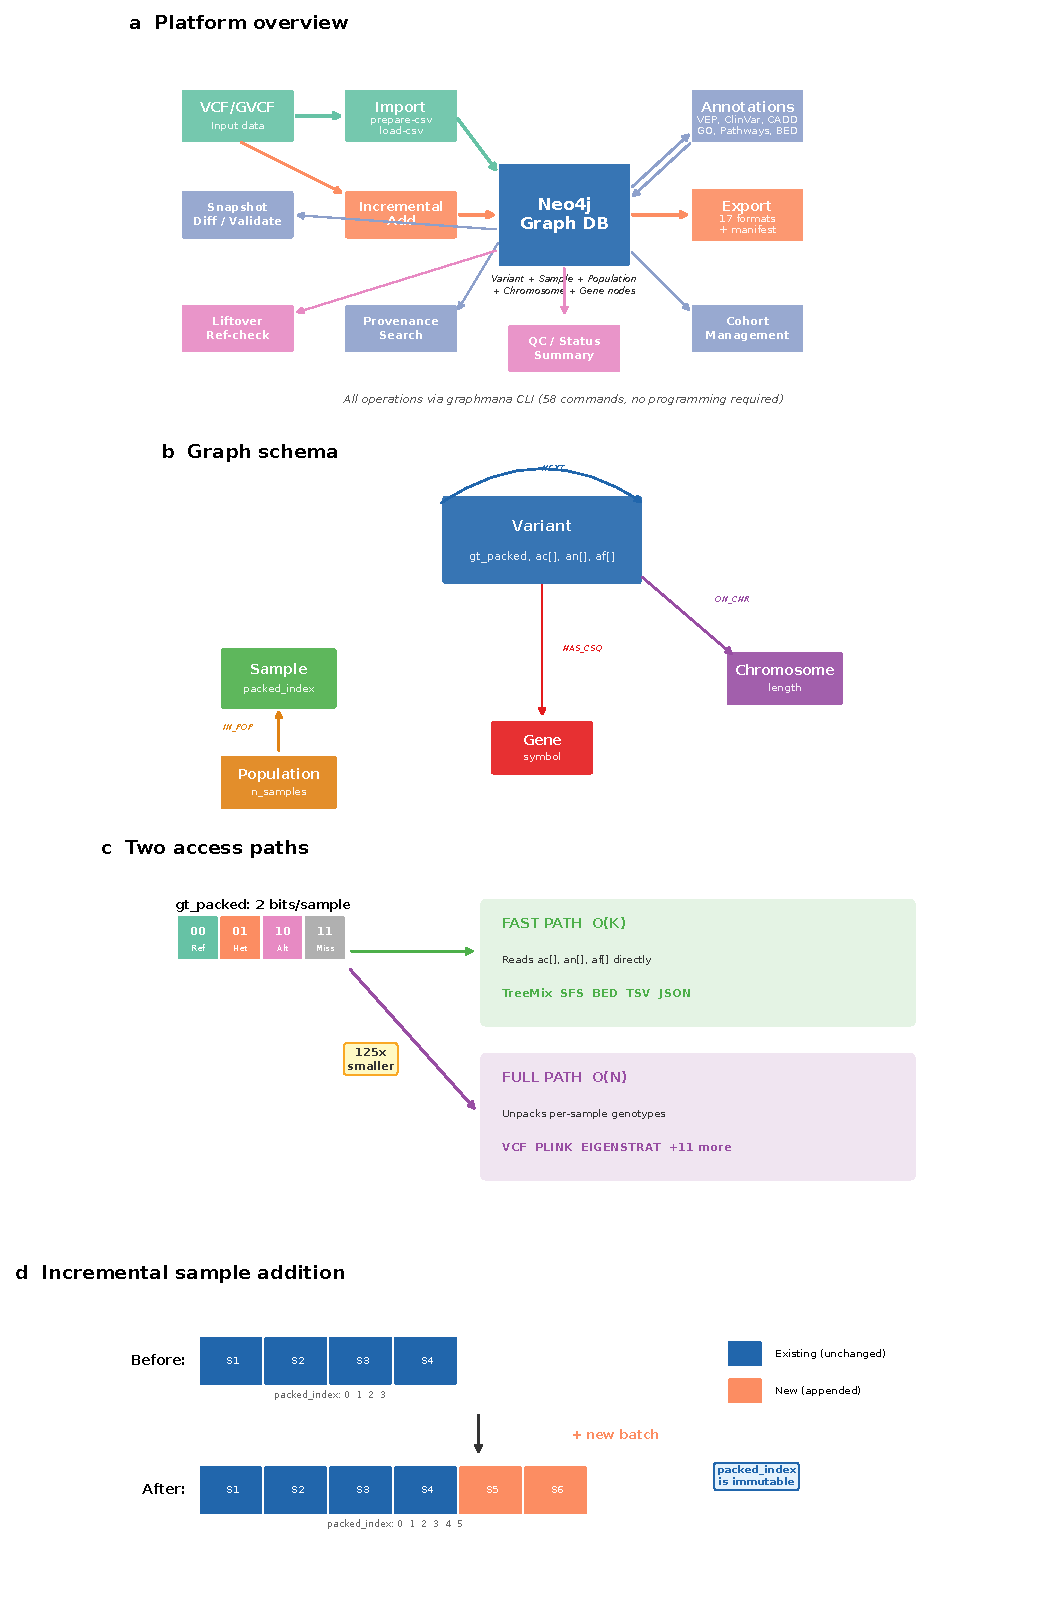
\includegraphics[width=\textwidth]{figures/fig1_architecture.pdf}
\caption{\textbf{GraphMana platform architecture.}
(\textbf{a})~System overview showing data flow from VCF input through a graph database to 17 export formats. Functional modules include annotation management, cohort definitions, provenance tracking, quality control, and database administration. All 58 CLI commands are organized into nine functional domains (Supplementary Fig.~1).
(\textbf{b})~Graph schema: five node types connected by typed relationships. Annotation updates modify edge properties independently of genotype data.
(\textbf{c})~Two access paths: FAST PATH queries pre-computed population arrays in $O(K)$ time; FULL PATH unpacks per-sample genotypes in $O(N)$ time.
(\textbf{d})~Incremental sample addition: new genotypes appended to packed arrays; immutable packed\_index ensures downstream reference stability.}
\label{fig:architecture}
\end{figure}

%% --- Discussion point 3: Figure 2 — removed Panel c ---
\begin{figure}[h]
\centering
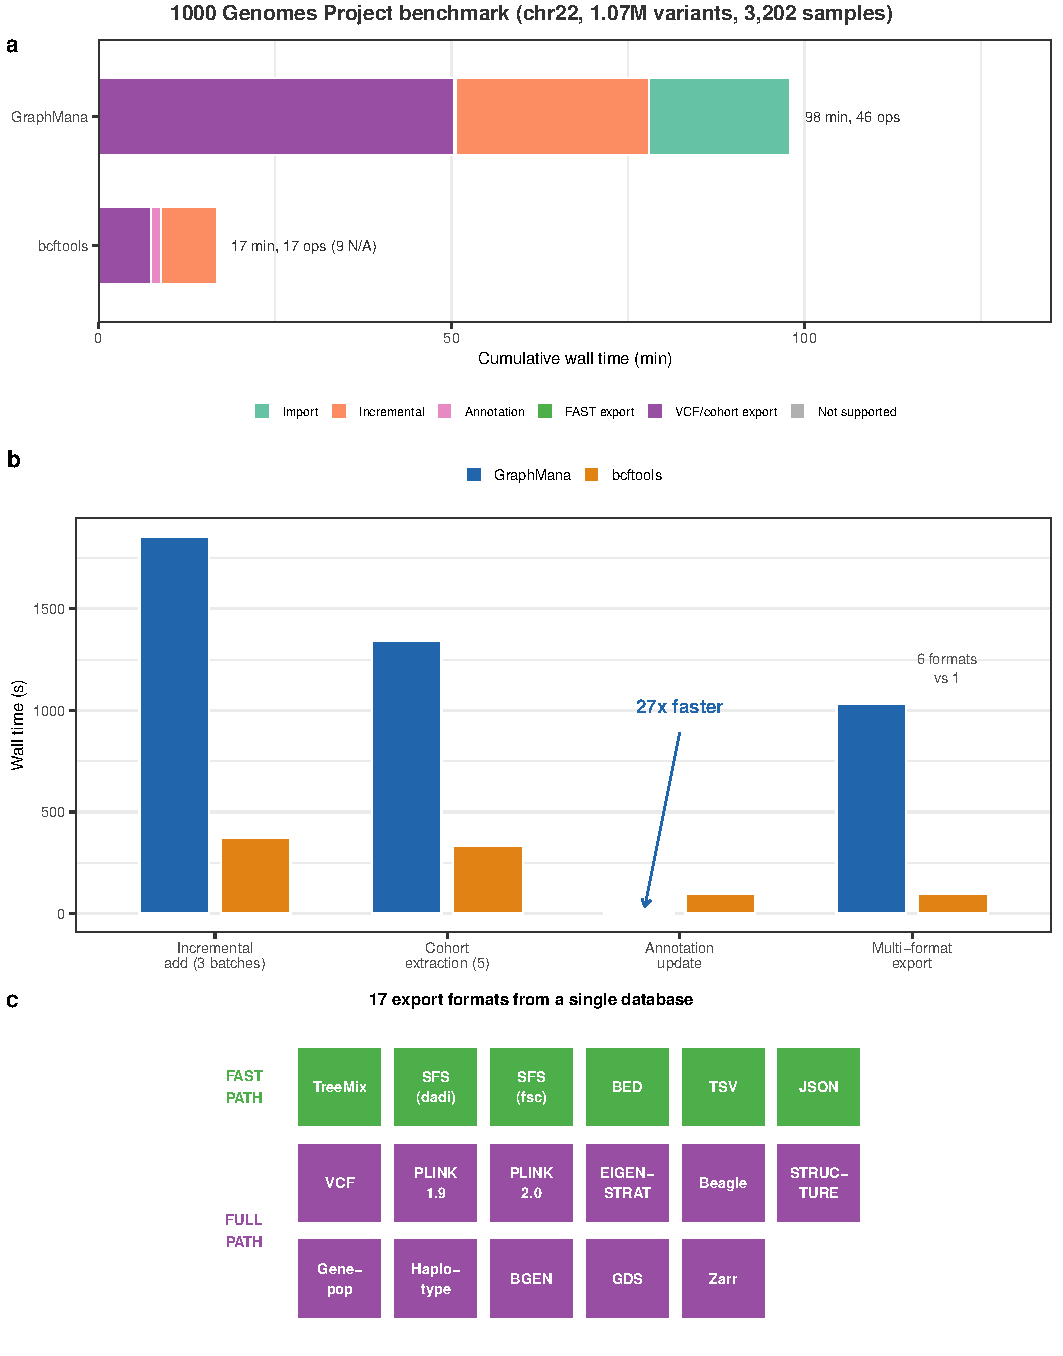
\includegraphics[width=\textwidth]{figures/fig2_benchmark_ggplot.pdf}
\caption{\textbf{Benchmark comparison on 1000 Genomes Project chromosome~22} (1.07M variants, 3,202 human whole-genome samples).
(\textbf{a})~Lifecycle simulation: GraphMana completes 46 operations from a persistent database; bcftools completes 17 of 26 (9 require additional tools, shown in grey). Time difference reflects graph database query overhead offset by elimination of format regeneration.
(\textbf{b})~Per-task comparison. bcftools is faster for VCF-centric operations. GraphMana achieves a 27-fold speedup for annotation updates through in-place edge modification, and provides multi-format export (6 formats) where bcftools supports only VCF.}
\label{fig:benchmark}
\end{figure}

%% ======================================================================
%% ONLINE METHODS
%% ======================================================================

\section*{Online Methods}

\subsection*{Graph database technology for genomic data management}

Population genomics data is inherently a network of typed relationships: variants are located on chromosomes, samples belong to populations, genes carry functional consequences, and every operation has provenance. Conventional approaches store this network as flat files requiring manual relationship maintenance. A graph database stores data as nodes and edges with properties, traversing pre-materialized connections in constant time per hop. This property-graph model maps onto population genomics: a Variant node connects to Chromosome, Gene, and Population nodes via typed edges. Edges can be updated independently---an annotation update modifies edge properties without touching genotype data. A detailed introduction to graph database concepts for non-specialist readers is provided in Supplementary Note~4.

We note that graph databases are one of several possible architectures (Table~\ref{tab:architectures}). The graph-native approach was chosen because it co-locates relationship semantics with the data, making lifecycle operations inherently persistent. This representation also serves as the foundation for the companion GraphPop engine~\cite{graphpop}. GraphMana uses Neo4j Community Edition~\cite{neo4j} as its graph database engine; the design principles are not specific to Neo4j.

\subsection*{Software architecture}

GraphMana is implemented as a Python command-line application (21,267 lines) with a Java plugin (2,864 lines) for server-side procedures. The Python layer handles VCF parsing via cyvcf2~\cite{pedersen2017cyvcf2}, genotype packing via NumPy (complementing scikit-allel~\cite{scikitallel}), CSV generation, and all export format writers. The 58 CLI commands are organized into nine functional domains (Supplementary Fig.~1). A companion Python package provides a Jupyter-compatible API. The test suite comprises 1,439 unit and integration tests.

\subsection*{Graph schema and data encoding}

The graph contains five node types: Variant, Sample, Population, Chromosome, and Gene, connected by typed relationships (ON\_CHROMOSOME, IN\_POPULATION, HAS\_CONSEQUENCE, NEXT). Variant nodes store genotype data as packed byte arrays: gt\_packed (2 bits per sample), phase\_packed (1 bit per sample), and ploidy\_packed (1 bit per sample). This stores 4 genotypes per byte, achieving a 125-fold reduction versus per-sample edges (Supplementary Table~6). Each Variant also carries $K$-element population arrays (ac, an, af, het\_count, hom\_alt\_count, het\_exp) that are constant size regardless of $N$. Full encoding details are provided in Supplementary Note~2.

\subsection*{Import pipeline}

GraphMana uses a two-step split pipeline. The prepare-csv step parses VCFs, packs genotypes, computes population statistics, and writes CSV files (embarrassingly parallel, no database needed). The load-csv step uses the database engine's bulk import. On our benchmark hardware (32 cores, 64~GB RAM, NVMe SSD), CSV generation for 2,500 human whole-genome samples across 22 chromosomes (70.7M variants) completed in 95 minutes with 16 threads; bulk loading completed in 3 minutes.

\subsection*{Incremental sample addition}

New samples are added by extending packed genotype arrays. Three strategies are provided: Cypher transactions, export-extend-reimport, and CSV-to-CSV rebuild. The CSV-to-CSV path extended 70.7M variants with 234 samples in 182 minutes; approximately 95\% required only HomRef extension.

\subsection*{Correctness validation}

We validated genotype fidelity by roundtrip (import $\to$ VCF export $\to$ comparison), achieving 99.999\%+ concordance. A systematic correctness matrix is in Supplementary Tables~10--11.

\subsection*{Benchmark methodology}

All benchmarks used the 1000 Genomes Project~\cite{byrska2022} (GRCh38). Chromosome 22 (1,066,557 variants, 3,202 samples, 26 populations) served as the primary target. We compared against bcftools~\cite{danecek2021bcftools} (v1.17) across five benchmarks. Per-operation timings favor bcftools; GraphMana's advantage lies in avoiding repeated regeneration.

%% --- Discussion point 1: Clarify human WGS ---
\subsection*{Scalability}

Storage per variant is $\lceil N/4 \rceil$ bytes for genotypes and $\lceil N/8 \rceil$ bytes for phase. All scaling estimates assume human whole-genome data ($\sim$85M biallelic variants); for species or designs with fewer variants, requirements scale proportionally (Supplementary Tables~6--7). At biobank scale, distributed frameworks are more appropriate.

\subsection*{Deployment}

GraphMana runs on workstations and HPC cluster nodes via a two-step split pipeline. SLURM and PBS job scripts are provided. The database must reside on local SSD.

%% ======================================================================
\backmatter

\section*{Data availability}

GraphMana is available at \url{https://github.com/jfmao/GraphMana} under the MIT license. Benchmark data and pre-built databases are deposited at \url{https://doi.org/[to be assigned upon acceptance]}.

\section*{Code availability}

All source code is at \url{https://github.com/jfmao/GraphMana} under the MIT license.

\bmhead{Acknowledgements}

This work was supported by [funding sources to be completed]. The 1000 Genomes Project dataset~\cite{byrska2022} was used under its open data access terms.

\bmhead{Author contributions}

J.M.\ conceived the project, designed and implemented the software, performed benchmarks, and wrote the manuscript.

\section*{Competing interests}

The author declares no competing interests.

%% ======================================================================
%% REFERENCES
%% ======================================================================

\begin{thebibliography}{15}

\bibitem{graphpop}
Mao, J. GraphPop: graph-native population genomics with annotation-conditioned queries. \textit{Nature Methods} (companion paper, in preparation).

\bibitem{neo4j}
Neo4j, Inc. Neo4j Graph Database. \url{https://neo4j.com} (Community Edition 5.x).

\bibitem{byrska2022}
Byrska-Bishop, M. et al. High-coverage whole-genome sequencing of the expanded 1000 Genomes Project cohort including 602 trios. \textit{Cell} \textbf{185}, 3426--3440.e19 (2022).

\bibitem{hail}
Hail Team. Hail: An Open-Source Framework for Scalable Genomic Data Analysis. \url{https://hail.is}.

\bibitem{chang2015plink}
Chang, C.C. et al. Second-generation PLINK: rising to the challenge of larger and richer datasets. \textit{GigaScience} \textbf{4}, s13742-015-0047-8 (2015).

\bibitem{danecek2021bcftools}
Danecek, P. et al. Twelve years of SAMtools and BCFtools. \textit{GigaScience} \textbf{10}, giab008 (2021).

\bibitem{scikitallel}
Miles, A. et al. scikit-allel: A Python package for exploring and analysing genetic variation data. \url{https://github.com/cggh/scikit-allel}.

\bibitem{pedersen2017cyvcf2}
Pedersen, B.S. \& Quinlan, A.R. cyvcf2: fast, flexible variant analysis with Python. \textit{Bioinformatics} \textbf{33}, 1867--1869 (2017).

\bibitem{danecek2011vcf}
Danecek, P. et al. The variant call format and VCFtools. \textit{Bioinformatics} \textbf{27}, 2156--2158 (2011).

\bibitem{gutenkunst2009dadi}
Gutenkunst, R.N. et al. Inferring the joint demographic history of multiple populations from multidimensional SNP frequency data. \textit{PLoS Genetics} \textbf{5}, e1000695 (2009).

\bibitem{excoffier2021fsc}
Excoffier, L. et al. fastsimcoal2: demographic inference under complex evolutionary scenarios. \textit{Bioinformatics} \textbf{37}, 4882--4885 (2021).

\bibitem{pickrell2012treemix}
Pickrell, J.K. \& Pritchard, J.K. Inference of population splits and mixtures from genome-wide allele frequency data. \textit{PLoS Genetics} \textbf{8}, e1002967 (2012).

\bibitem{patterson2006eigenstrat}
Patterson, N., Price, A.L. \& Reich, D. Population structure and eigenanalysis. \textit{PLoS Genetics} \textbf{2}, e190 (2006).

\bibitem{browning2007beagle}
Browning, S.R. \& Browning, B.L. Rapid and accurate haplotype phasing and missing-data inference for whole-genome association studies by use of localized haplotype clustering. \textit{Am.\ J.\ Hum.\ Genet.} \textbf{81}, 1084--1097 (2007).

\bibitem{pritchard2000structure}
Pritchard, J.K., Stephens, M. \& Donnelly, P. Inference of population structure using multilocus genotype data. \textit{Genetics} \textbf{155}, 945--959 (2000).

\end{thebibliography}

\end{document}
